\chapter{Implementation}
\label{chap:implementation}

The previous chapter established the methodological framework and the operational requirements for the anomaly detection system. This chapter details the technical realization of these concepts, focusing on the software stack, the integration into the Azure ecosystem, and the internal orchestration logic of the Scala microservice and the Python analytics endpoint.

\section{Integrated System Architecture and Technology Stack}

The implementation utilizes a polyglot approach to leverage the specific strengths of different programming paradigms. While the orchestration and data processing are handled by a Scala microservice to ensure high-performance parallelism, the predictive modeling is realized through a Python endpoint optimized for machine learning.

\subsection{Deployment and Cluster Integration}

The system is designed as a modular Docker container that operates within the same Azure Kubernetes Services (AKS) cluster as the core Eliona microservices. This co-location ensures low-latency communication between the detection logic and the primary data storage. The architecture remains environment-agnostic; for on-premise deployments, the entire stack, including the analytics endpoint, can be executed locally as a suite of interconnected containers.

\begin{figure}[htbp]
	\centering
	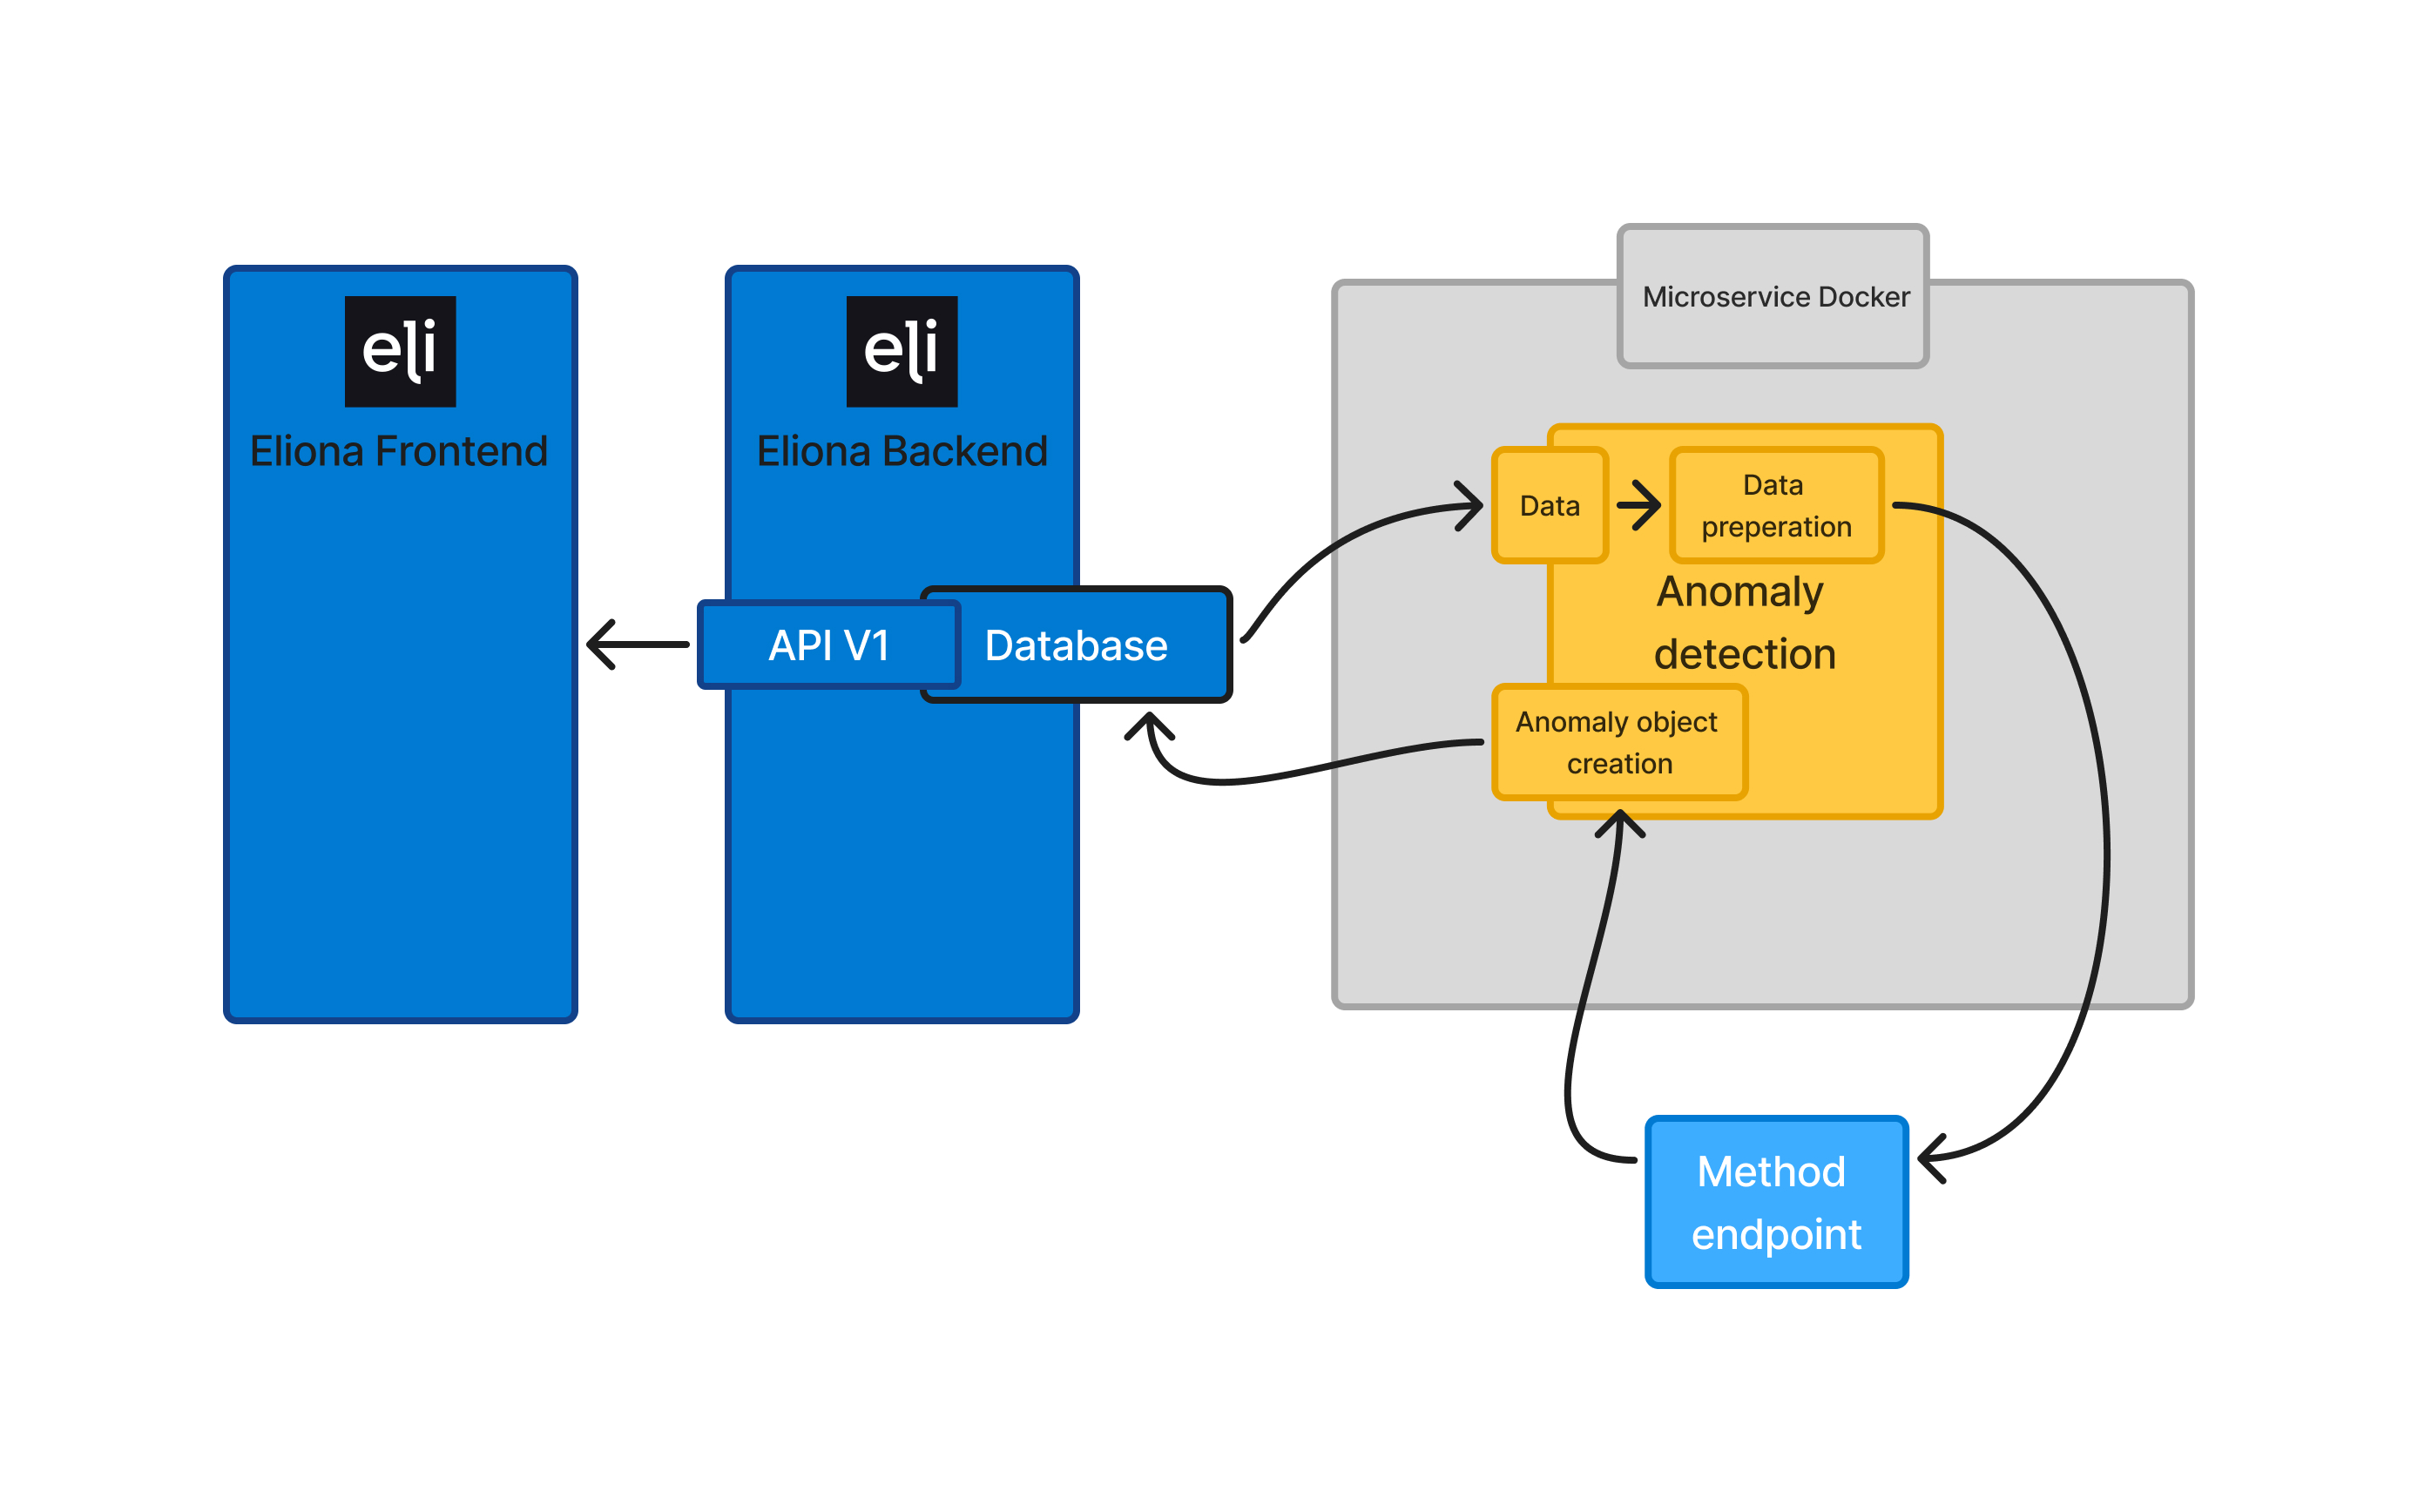
\includegraphics[width=1.0\textwidth]{images/first-high-level-architecture.jpg}
	\caption{High-level deployment of the anomaly detection microservice and Python analytics endpoint within the Eliona and Azure ecosystems.}
	\label{fig:implementation-architecture}
\end{figure}

\subsection{Data Orchestration and Persistence}

The microservice establishes a closed-loop data pipeline with the Eliona backend:

\begin{description}
	\item[Ingestion] Telemetry data is retrieved directly from the centralized PostgreSQL/TimescaleDB instance.
	\item[Analytics loop] After performing data preparation, the microservice transmits multivariate tensors to the method endpoint.
	\item[Synthesis and storage] If the returned predictions indicate a deviation, the service creates an anomaly object. These objects are persisted in the database, where they become accessible to the Eliona frontend via API~V1 for visualization and reporting.
\end{description}

\section{Chronos-2 Analytics Endpoint}

The analytical core is implemented as a dedicated Python microservice hosting the
Chronos-2 transformer model. The service processes batched multivariate time series,
receiving historical context and exogenous covariates and returning probabilistic
quantile forecasts that define the regime-conditioned normative envelope.

For production deployment, the service is exposed as a managed online endpoint in
Azure Machine Learning. This provides automated horizontal scaling, versioned model
management, and containerized deployment, enabling seamless operation in both cloud
and on-premise environments while supporting non-stationary adaptation requirements.

\section{Scala Microservice: Multi-Tenant Orchestration}

System-wide orchestration is implemented as a dedicated Scala microservice that
coordinates data ingestion, contextual enrichment, anomaly scoring, and tenant-level
isolation. Predictive inference is delegated to the Python Chronos-2 endpoint, while
the Scala layer performs all asynchronous I/O, scheduling, and hierarchical
orchestration.

Scala is selected for its strong static typing and high-throughput concurrency model,
enabling safe parallel processing of large multivariate telemetry tensors and complex
building ontologies under multi-tenant operation.

\subsection{Multi-Tenant Lifecycle Management}

Tenants are managed through a centralized orchestration layer that enforces strict
logical isolation across organizations. Independent worker pipelines are instantiated
per tenant and operate on disjoint telemetry scopes, ensuring that ingestion,
processing, and anomaly attribution remain isolated across building portfolios.

Tenant lifecycles are synchronized periodically with licensing and configuration
state. Worker pipelines are automatically instantiated, restarted, or terminated in
response to tenant state changes, ensuring fault tolerance and consistent multi-tenant
operation without manual intervention.

\section{Data Acquisition and Processing Pipeline}

Raw building telemetry is transformed into structured model inputs through a
multi-stage pipeline that performs attribute selection, contextual enrichment, and
robust data conditioning.

\subsection{Attribute Selection and Hierarchical Scoping}

Energy-relevant telemetry channels are identified using semantic attribute metadata
and unit normalization. To ensure operational relevance and computational efficiency,
attributes with negligible economic impact are excluded. Anomaly detection is
performed on the upper hierarchy levels (aggregate and floor meters), while
subordinate assets are retained exclusively for diagnostic attribution.

\subsection{Contextual Enrichment}

External environmental drivers are incorporated via site-localized weather covariates
derived from geographical coordinates. This contextual enrichment enables
disambiguation between technical faults and demand variations induced by weather
conditions.

\subsection{Data Conditioning and Gap Resilience}

Telemetry is aggregated across multiple temporal resolutions and subjected to
gap-resilient conditioning. Transmission gaps and recovery artifacts are corrected
through redistribution mechanisms, while integrity flags preserve explicit data
quality context. Previously detected anomalous values are recursively imputed using
their predicted medians to prevent contamination of subsequent inference windows.

\subsection{Reactive Synchronization}

Model inputs are refreshed on a reactive schedule aligned with finalized aggregation
cycles, ensuring that inference is performed exclusively on complete and consistent
telemetry segments.

\section{Stochastic Inference and Anomaly Quantification}

Anomaly detection is performed by interpreting stochastic quantile forecasts
produced by Chronos-2 under a feature-driven inference strategy.

\subsection{Feature-Driven Inference}

To avoid sequential adaptation effects, inference is conditioned exclusively on
historical context and exogenous covariates (weather, occupancy, temporal indicators),
while the consumption value at the evaluated timestamp is withheld. This enforces
contextual rather than autoregressive normative modeling.

\subsection{Quantile-Based Scoring}

Requests are batched across meters and temporal resolutions. Chronos-2 returns
distribution-free quantile envelopes that define regime-conditioned normative bands.
Extreme quantiles define anomaly boundaries, while central quantiles serve as
conservative economic baselines.

An anomaly is triggered if the observation lies outside the extreme quantile envelope.
Signed deviations are measured relative to the central quantile to quantify waste
or savings under multimodal operating regimes. Deviations below a minimum economic
threshold are discarded to suppress negligible events.

\section{Hierarchical Root Cause Analysis (RCA)}

Upon detection of an aggregate-level anomaly, all subordinate assets in the functional
hierarchy are analyzed to localize the physical origin of the deviation.

\subsection{Diagnostic Attribution}

Sub-meter telemetry is re-evaluated to estimate asset-level financial contributions.
Impacts are attributed both at individual asset level and aggregated by semantic asset
categories (e.g., HVAC, lighting, plug loads), enabling identification of systematic
inefficiencies and dominant fault contributors.

\subsection{Localization and Contextual Enrichment}

Attributed root causes are enriched with spatial metadata and localized environmental
context to support interpretation and remediation planning.

\section{Temporal Collapse and Persistence}

Telemetry is evaluated across multiple temporal resolutions, which may generate
overlapping anomaly events. A temporal collapse mechanism consolidates lower-resolution
detections into higher-resolution events, preventing redundant alerts and preserving
the most conservative financial impact estimate across scales.

\section{AI Synthesis and Action Recommendation}

High-impact anomalies are forwarded to an interpretation layer that synthesizes
localized diagnostics, financial impact, and contextual metadata into structured
human-readable explanations and remediation recommendations using a domain-specialized
large language model (LLM). The LLM operates exclusively at the interpretation layer and
does not influence detection or scoring logic.

\section{Tenant-Specific Configuration}

Detection sensitivity, financial thresholds, and economic parameters are governed by
tenant-specific configuration profiles. These profiles enable adaptation to
organization-specific risk tolerance and energy pricing while preserving strict
multi-tenant isolation and auditability.




\section{Frontend Integration for Operational Decision Support}

The frontend constitutes the operational interface of the anomaly detection framework.
It exposes detected anomalies, quantified financial impact, hierarchical root causes,
and AI-synthesized recommendations in a multi-tenant environment, enabling human
validation and remediation workflows.

\subsection{Centralized Anomaly Registry and Validation Loop}

Detected anomalies are presented in a centralized registry that supports triage,
filtering, and prioritization by financial impact, severity, and affected assets
(Fig.~\ref{fig:anomaly-list}). Human operators can confirm or invalidate anomalies,
forming a controlled human-in-the-loop feedback channel. Invalidated anomalies are
excluded from future baseline construction to prevent contamination of normative
profiles.

\begin{figure}[htbp]
	\centering
	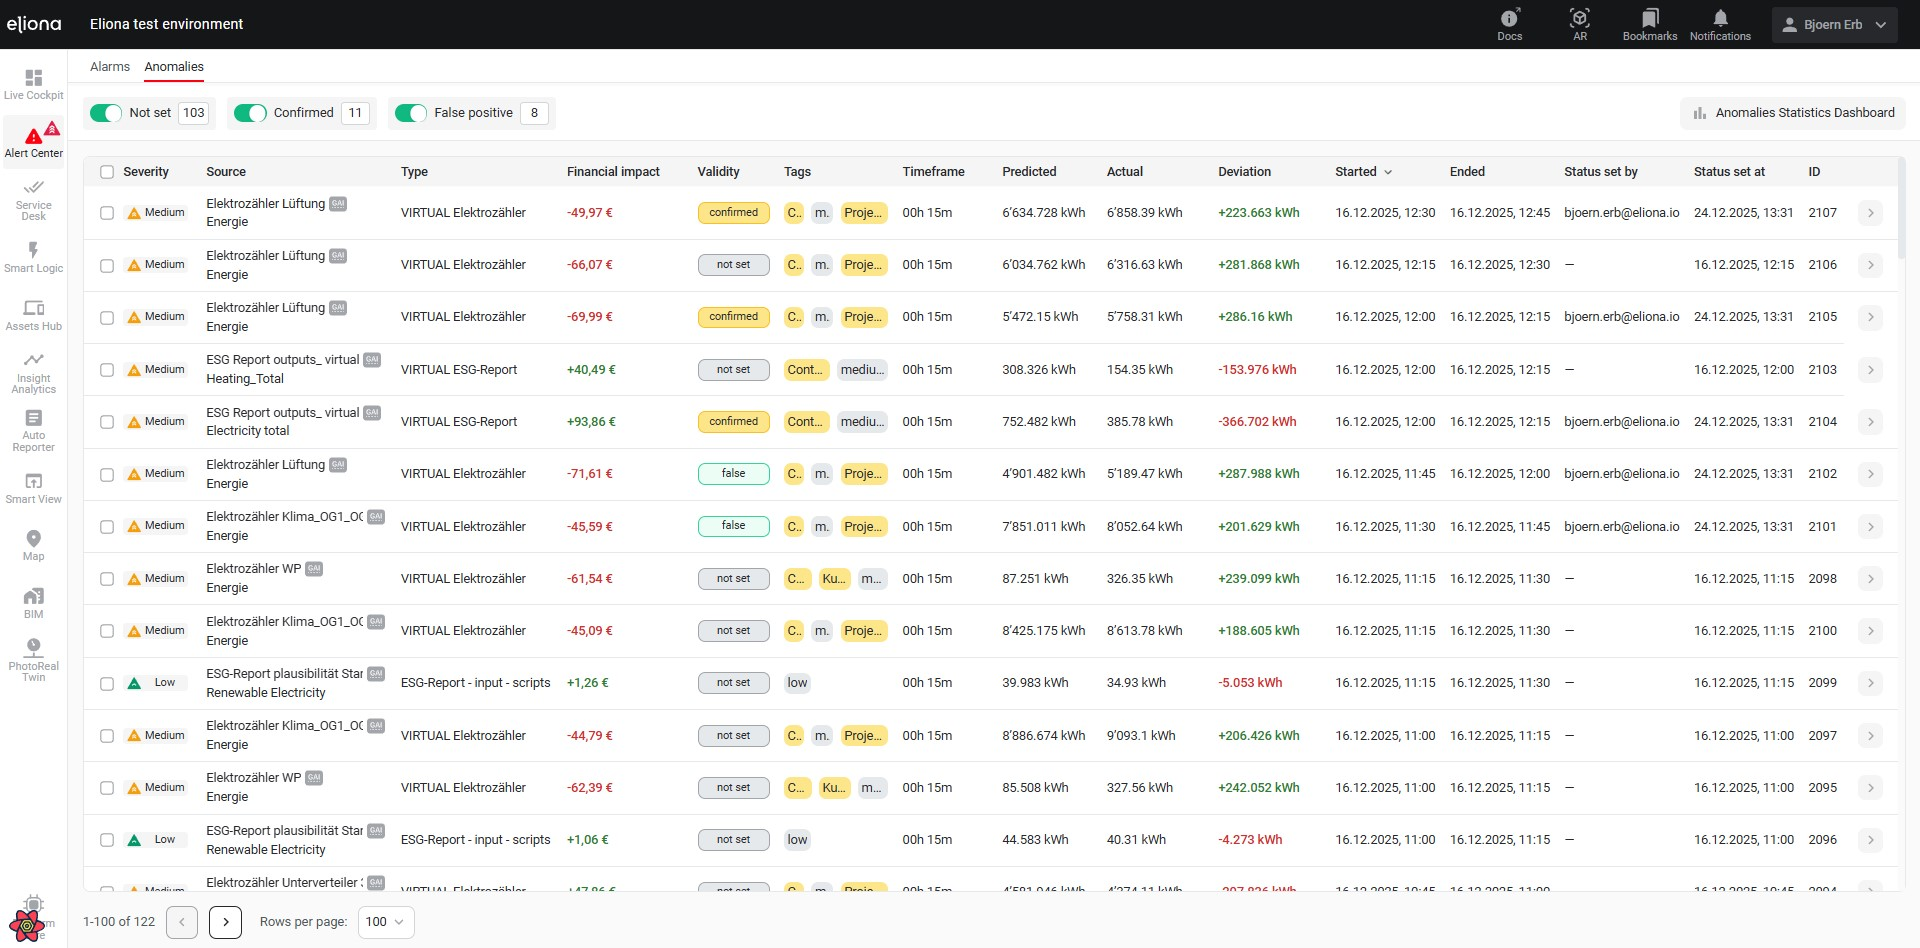
\includegraphics[width=1.0\textwidth]{images/anomaly-list.jpg}
	\caption{Central anomaly registry supporting prioritization, financial impact
	assessment, and validation workflows.}
	\label{fig:anomaly-list}
\end{figure}

\subsection{Quantile Visualization and Diagnostic Context}

Stochastic normative envelopes and anomalous deviations are visualized directly on
consumption charts using quantile-based uncertainty bands (Figs.~\ref{fig:anomalies-in-analytics}
and~\ref{fig:anomaly-analytic-dashboard}). These overlays enable severity assessment
relative to regime-conditioned baselines rather than absolute residual magnitudes.

\begin{figure}[htbp]
	\centering
	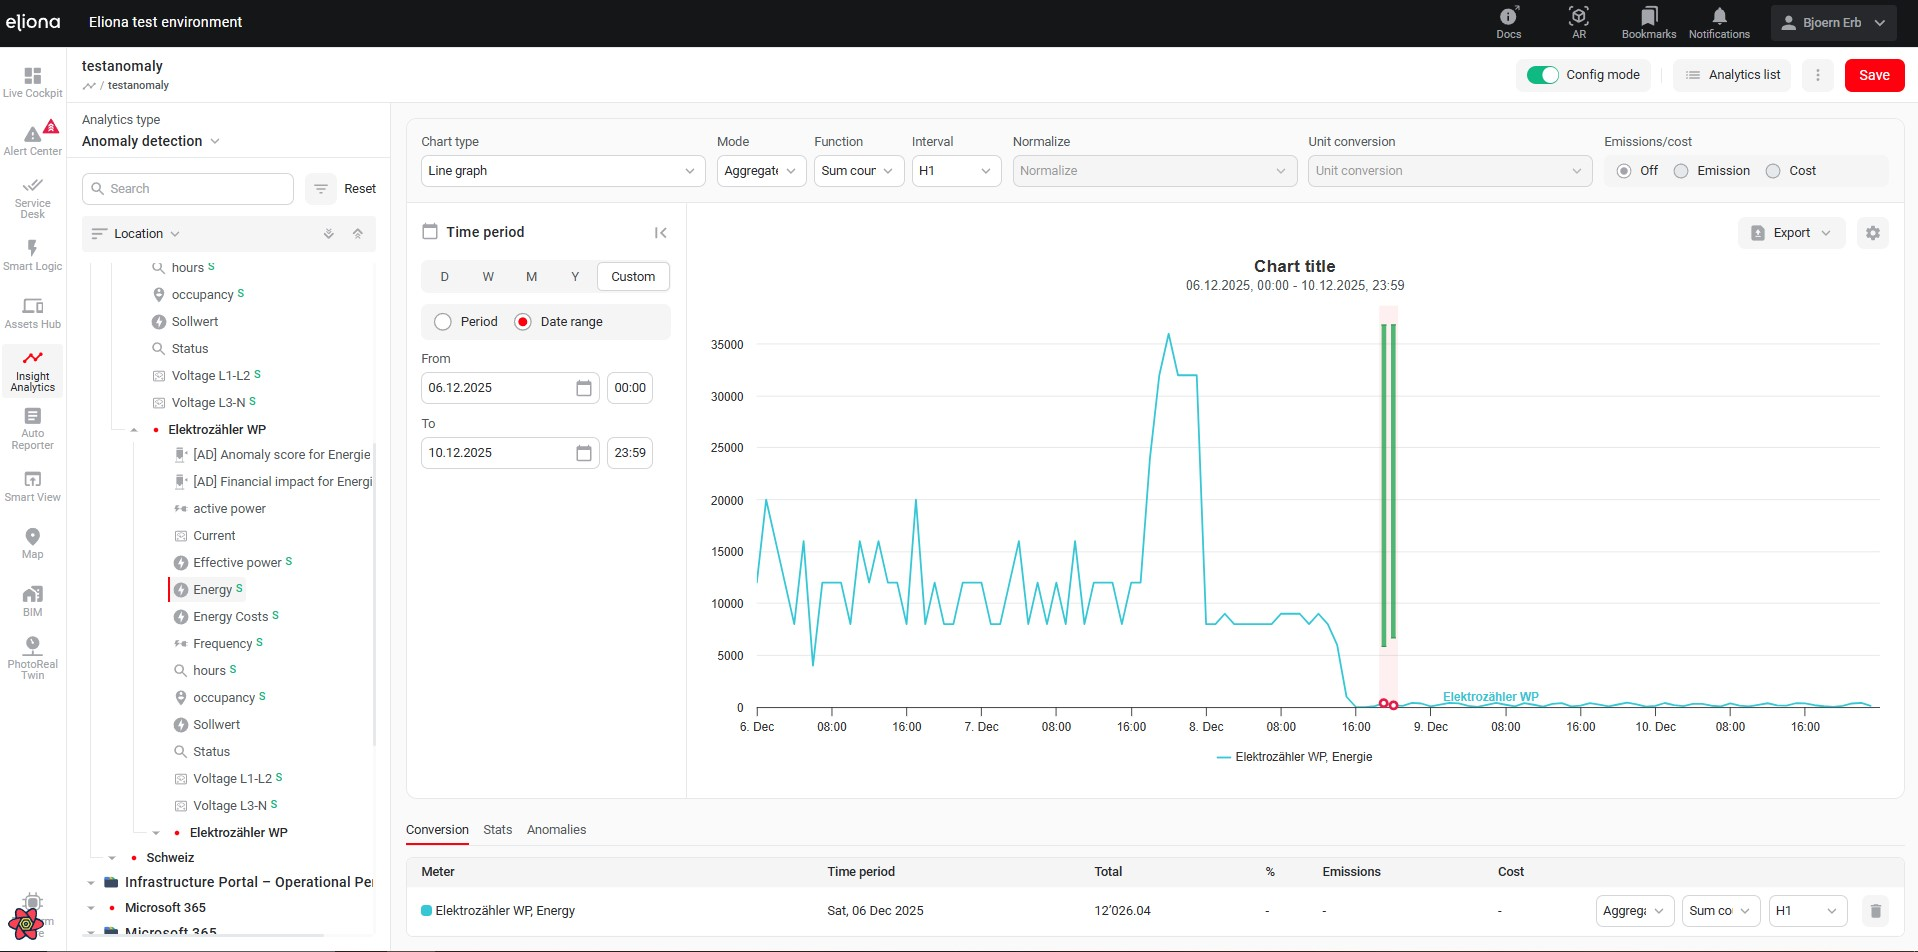
\includegraphics[width=1.0\textwidth]{images/anomalies-in-analytics.jpg}
	\caption{Quantile-based normative envelopes and anomaly overlays within analytics.}
	\label{fig:anomalies-in-analytics}
\end{figure}

\begin{figure}[htbp]
	\centering
	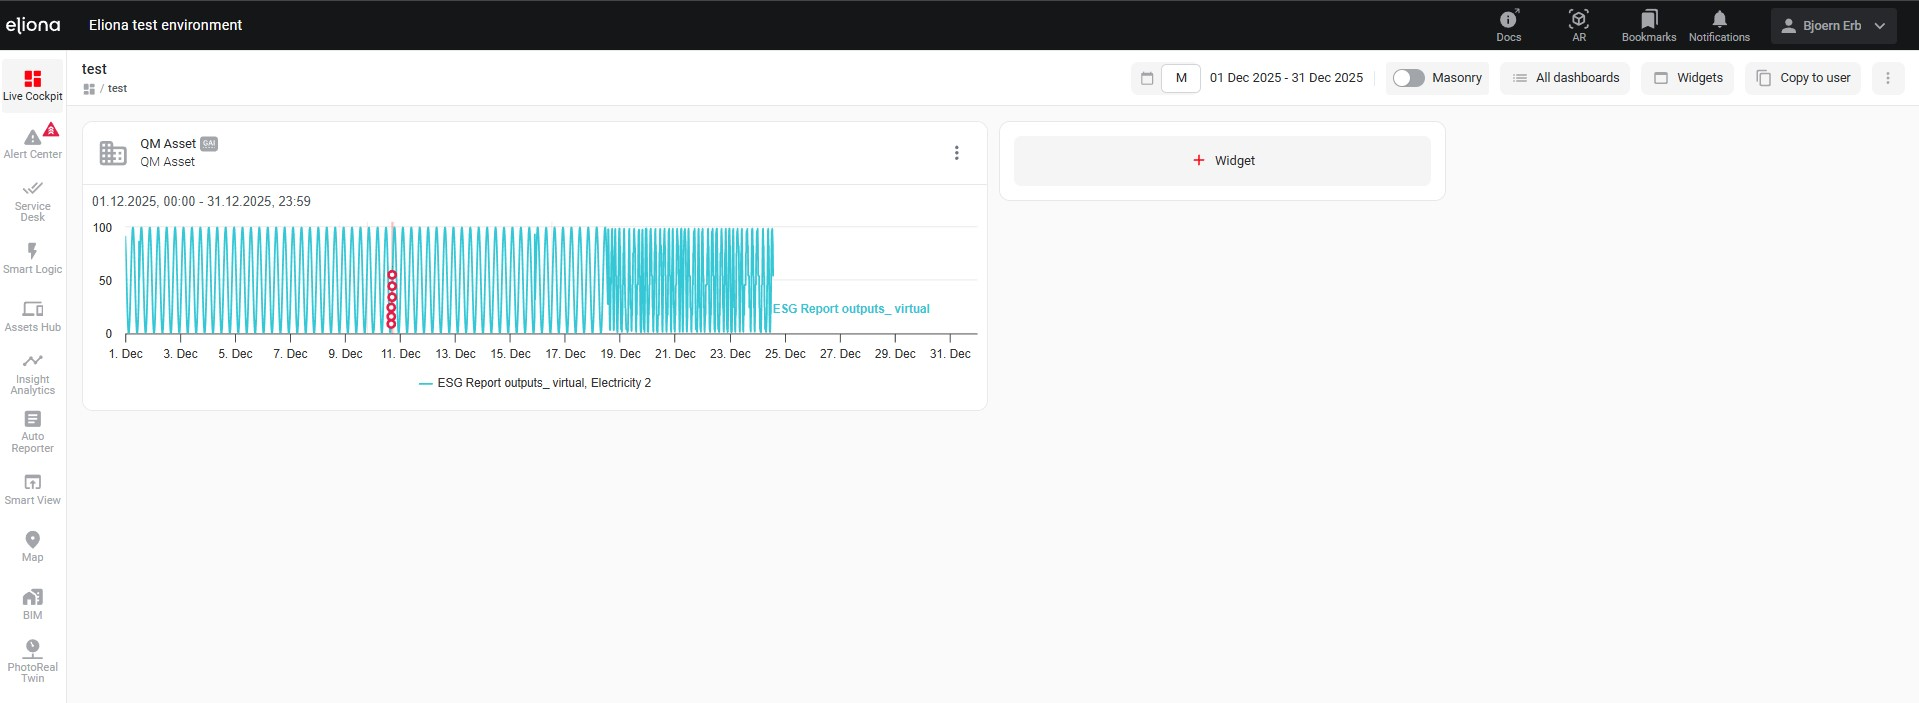
\includegraphics[width=1.0\textwidth]{images/anomaly-analytic-in-dashboard.jpg}
	\caption{Anomaly analytics embedded into operational dashboards.}
	\label{fig:anomaly-analytic-dashboard}
\end{figure}

\subsection{Contextual Tooltips and AI Synthesis}

Interactive tooltips expose localized financial impact, root cause attribution,
validation status, and AI-generated recommendations at individual anomalous points
(Fig.~\ref{fig:anomaly-tooltip}). This supports immediate contextual interpretation.

\begin{figure}[htbp]
	\centering
	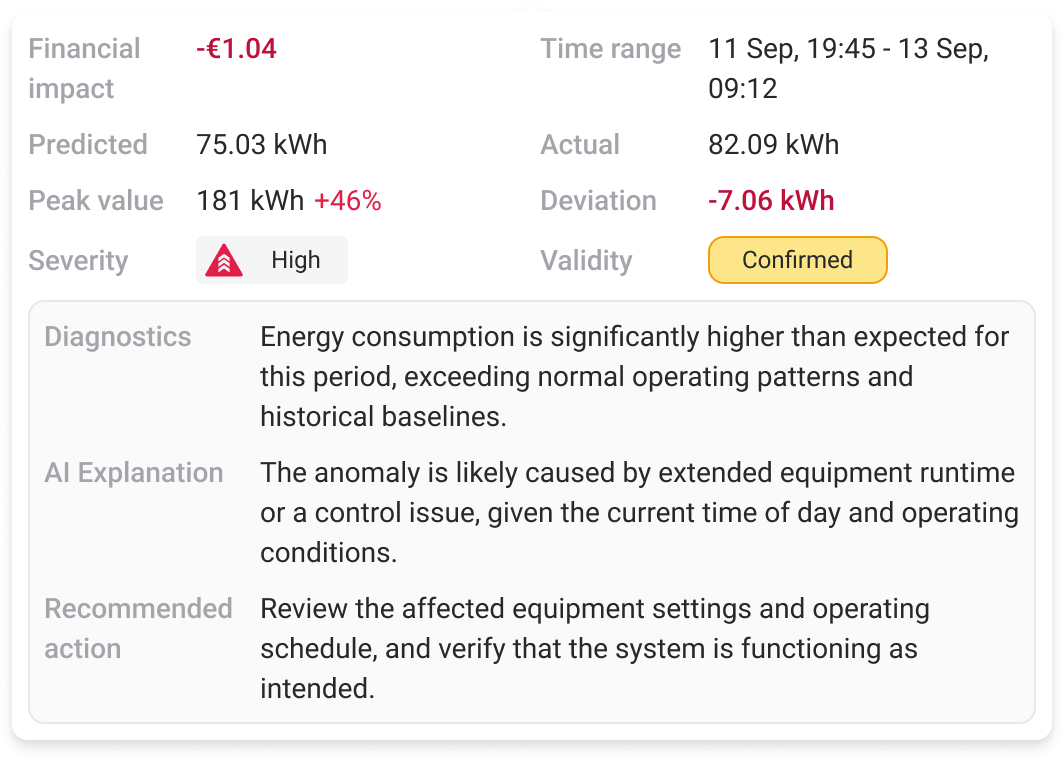
\includegraphics[width=0.8\textwidth]{images/Tooltip.png}
	\caption{Interactive diagnostic tooltip with financial impact and AI synthesis.}
	\label{fig:anomaly-tooltip}
\end{figure}

\subsection{Anomaly Detail View and Action Synthesis}

A dedicated anomaly detail view consolidates quantitative metrics, hierarchical root
causes, contextual metadata, and AI-generated remediation guidance into a single
operational workspace (Fig.~\ref{fig:anomaly-detail-view}), enabling transition from
detection to remediation.

\begin{figure}[htbp]
	\centering
	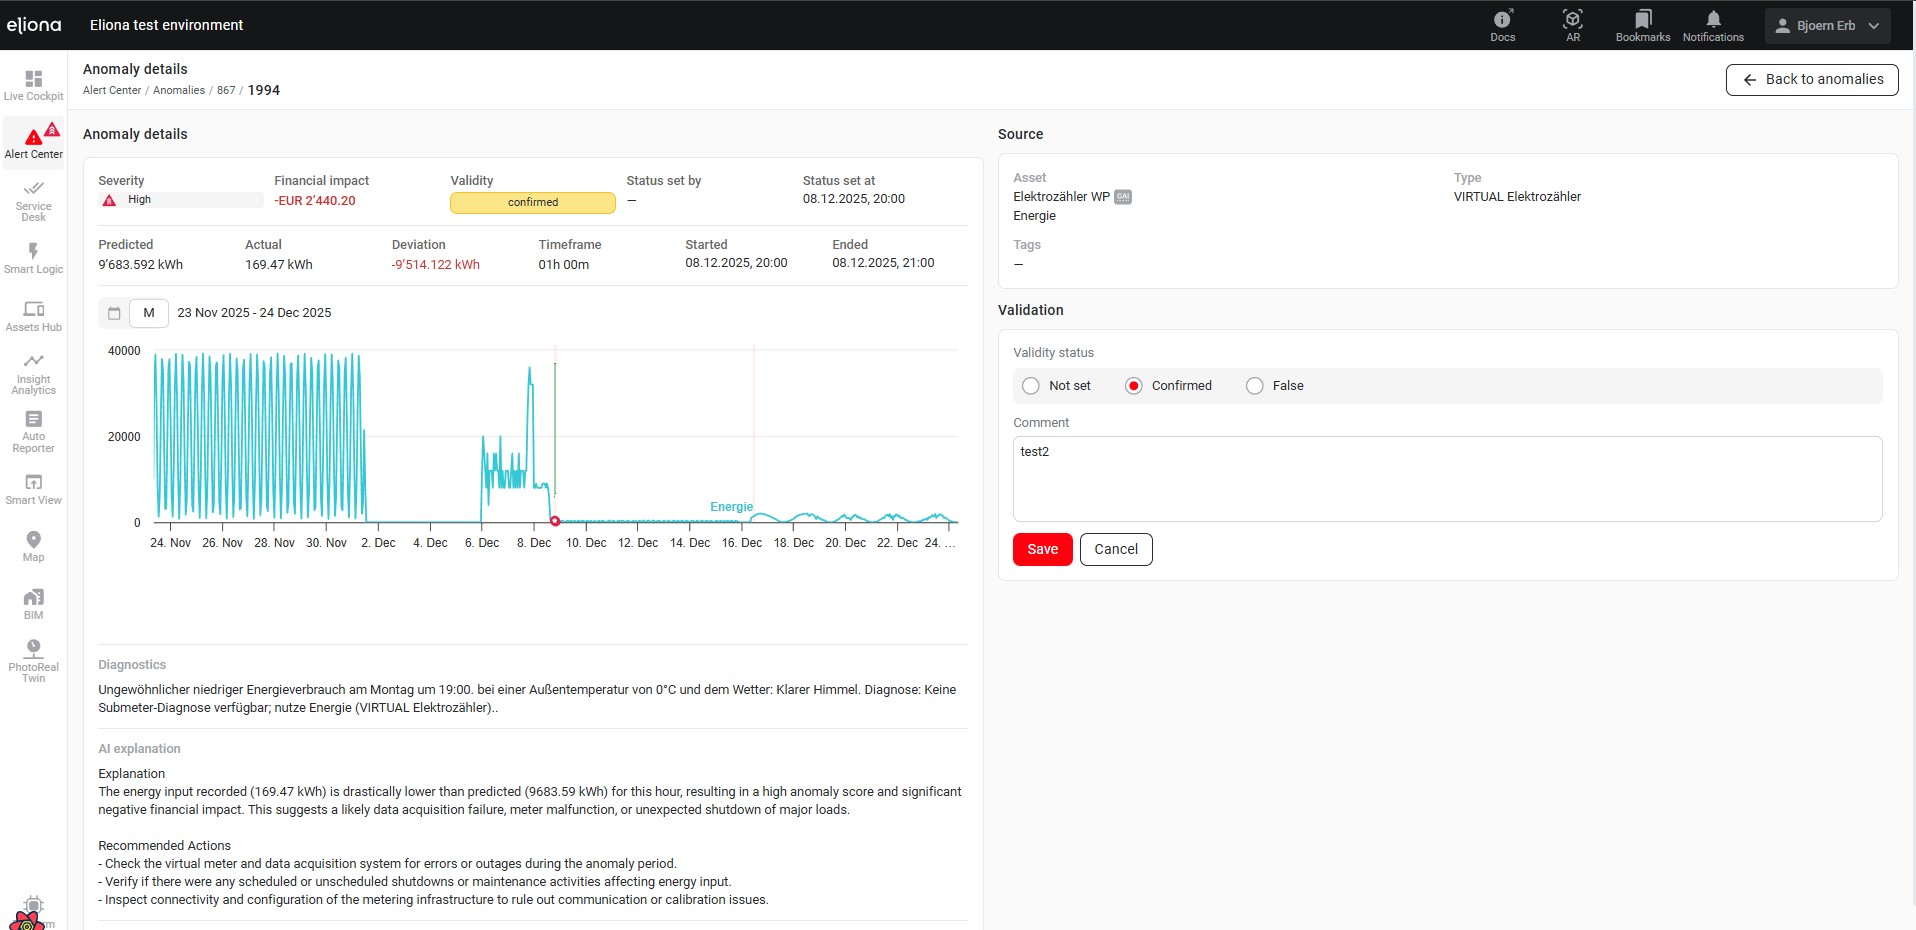
\includegraphics[width=1.0\textwidth]{images/anomaly-details-page.jpg}
	\caption{Integrated anomaly detail view combining financial impact, diagnostics, and
	AI-generated recommendations.}
	\label{fig:anomaly-detail-view}
\end{figure}

\subsection{Macro-Level Reporting and Portfolio Analytics}

Portfolio-level dashboards aggregate anomalies across tenants and sites, providing
executive visibility into financial impact, dominant asset categories, and temporal
patterns (Fig.~\ref{fig:anomaly-statistics-dashboard}). Heatmap visualizations reveal
systematic operational inefficiencies across time-of-day and day-of-week regimes.

\begin{figure}[htbp]
	\centering
	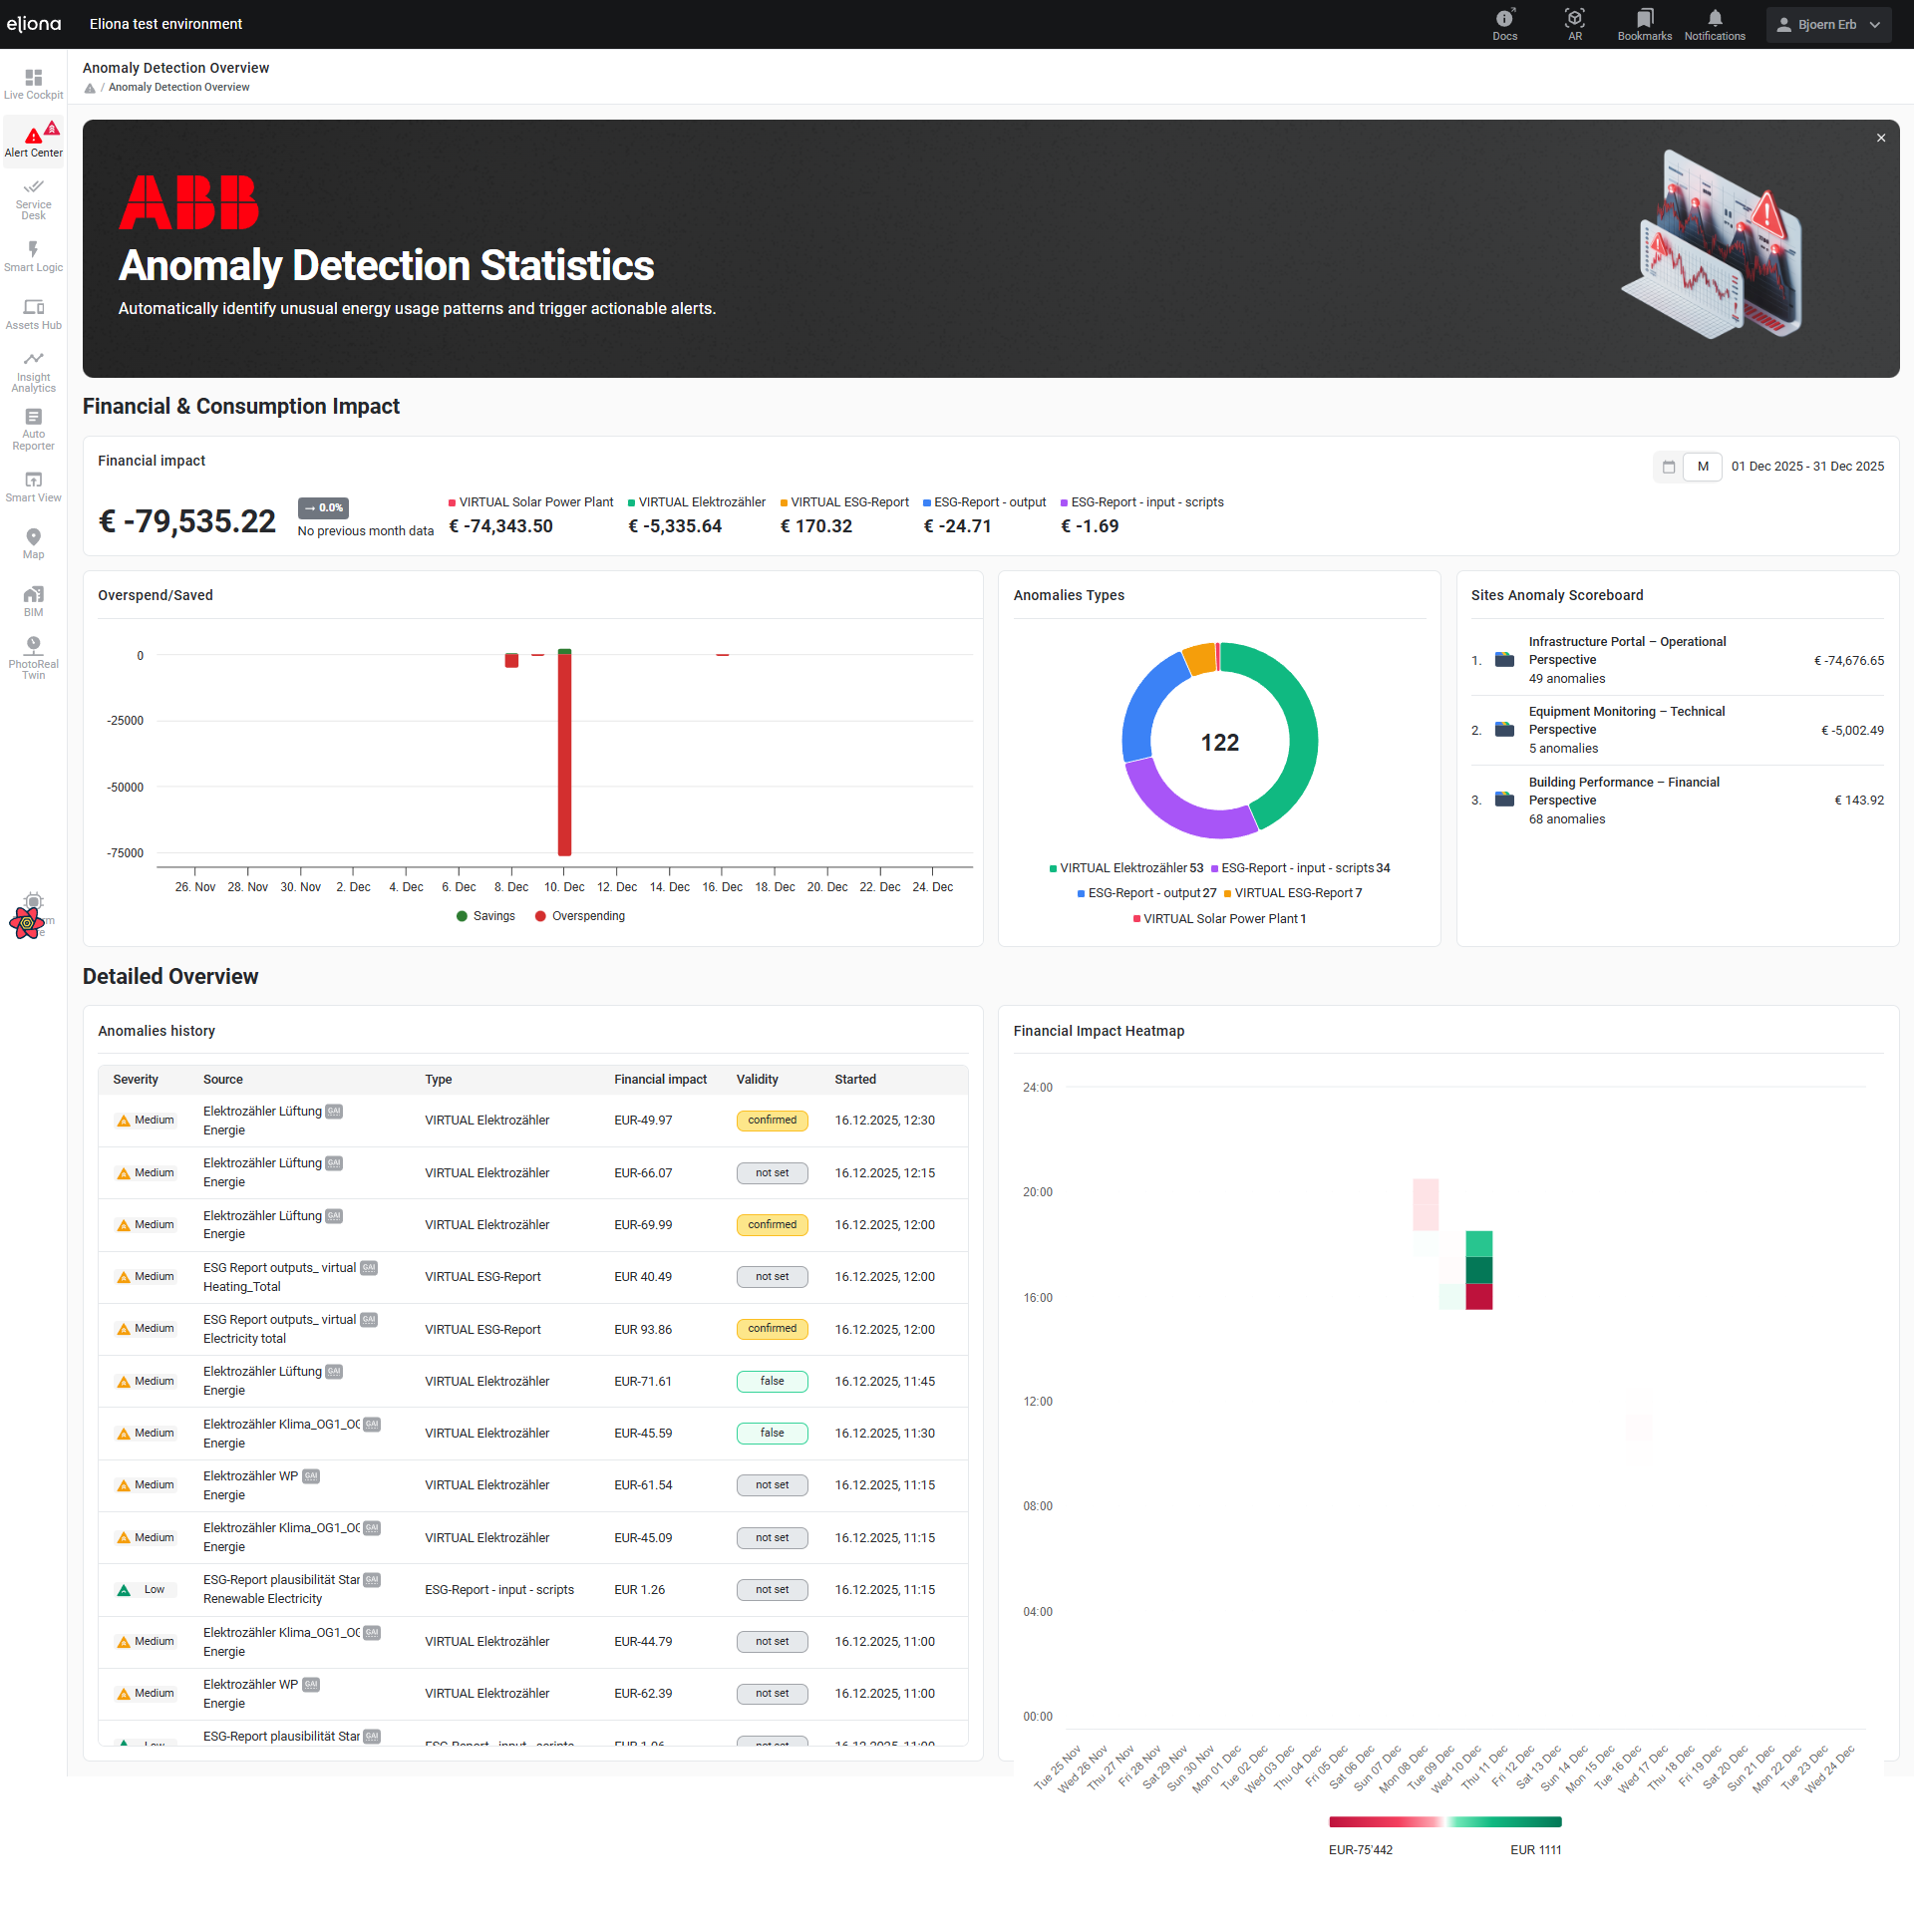
\includegraphics[width=1.0\textwidth]{images/anomalies-statistic-dashboard.png}
	\caption{Portfolio-level anomaly analytics and financial impact aggregation.}
	\label{fig:anomaly-statistics-dashboard}
\end{figure}

\subsection{Asset-Scoped Anomaly Integration}

Anomalies are integrated into asset detail views to support localized diagnostics and
historical inspection of deviations at the equipment and zone level
(Fig.~\ref{fig:anomalies-asset-details}).

\begin{figure}[htbp]
	\centering
	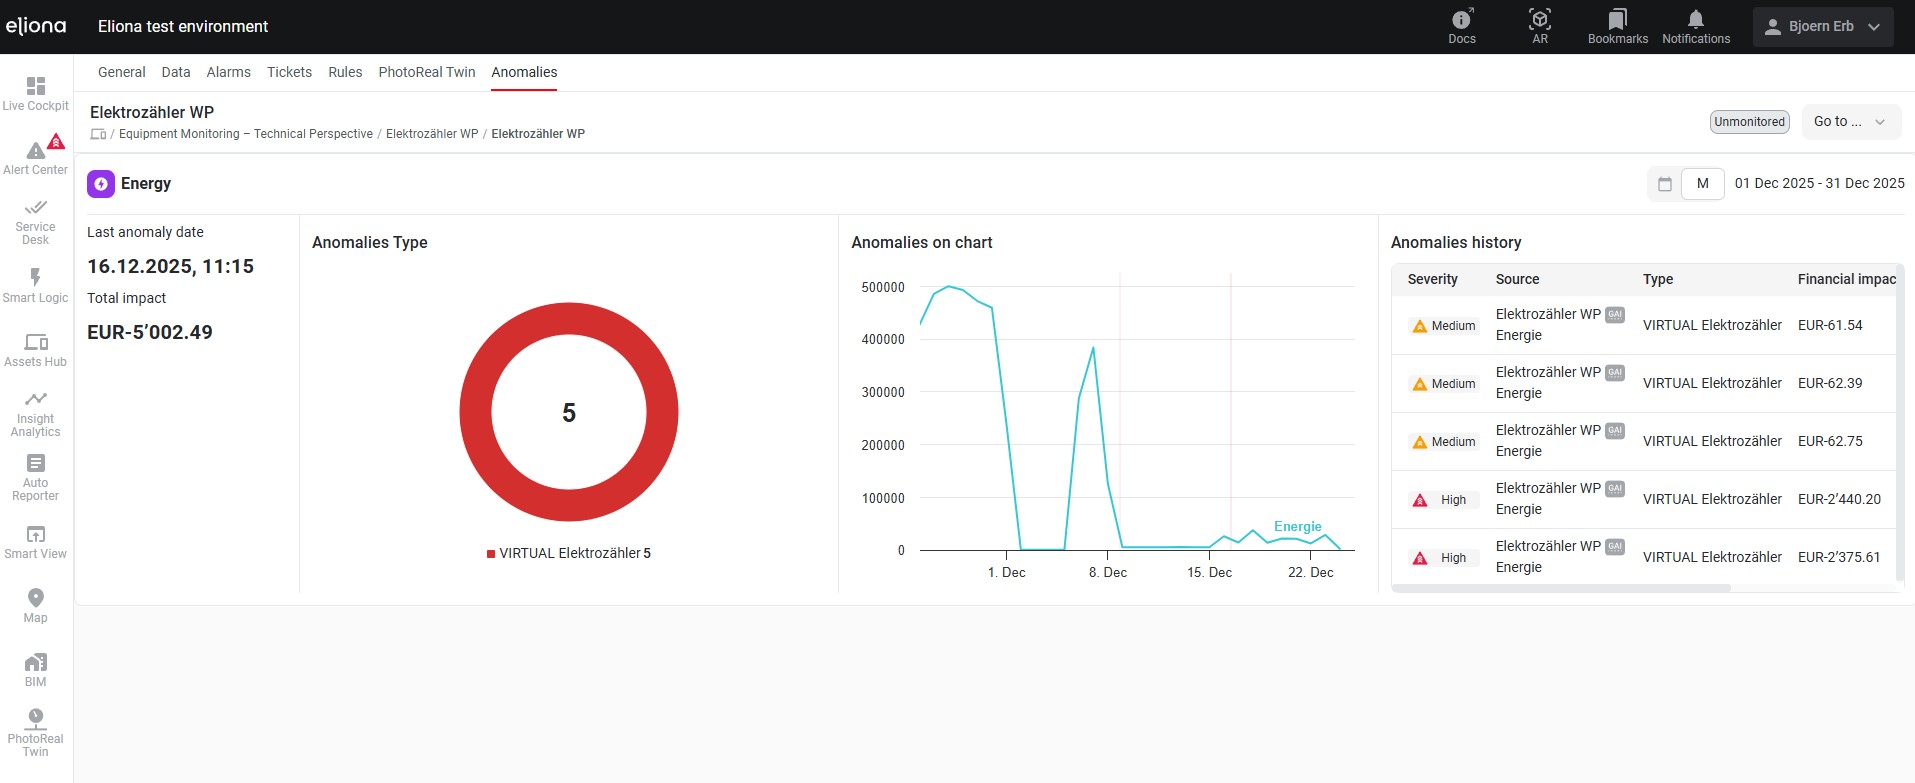
\includegraphics[width=1.0\textwidth]{images/anomalies-in-asset-details.jpg}
	\caption{Asset-level anomaly integration enabling localized inspection and triage.}
	\label{fig:anomalies-asset-details}
\end{figure}

\section{Implementation Summary}
The realized system fulfills the formal design objectives by providing an infinitely
scalable, cloud-native multi-tenant architecture for portfolio-scale building
monitoring. It performs stochastic multivariate anomaly detection using
distribution-free quantile modeling, accurately capturing multimodality and intrinsic
uncertainty in non-stationary energy telemetry.

The system adapts continuously to evolving operational regimes while preventing
persistent anomalies from being absorbed into normative baselines through explicit
human validation mechanisms. Detected deviations are translated into conservative
financial impact estimates, visualized through interpretable uncertainty envelopes,
and localized via hierarchical root cause analysis. A domain-specialized large language
model further synthesizes diagnostic evidence into actionable operational insights,
completing an end-to-end, economically interpretable anomaly management pipeline.
